\documentclass{beamer}
\usepackage{tcolorbox}
\usepackage{forloop}
\usepackage{bm}

\usepackage{mathtools}
\DeclarePairedDelimiter\ceil{\lceil}{\rceil}
\DeclarePairedDelimiter\floor{\lfloor}{\rfloor}

%\beamerdefaultoverlayspecification{<+->}
\newcommand{\data}{\mathcal{D}}

\DeclareMathOperator*{\argmin}{arg\,min}

\newcommand\Item[1][]{%
	\ifx\relax#1\relax  \item \else \item[#1] \fi
	\abovedisplayskip=0pt\abovedisplayshortskip=0pt~\vspace*{-\baselineskip}}

\usetheme{metropolis}           % Use metropolis theme


\title{Forecasting}
\date{\today}
\author{Nipun Batra}
\institute{IIT Gandhinagar}
\begin{document}
  \maketitle
  
  
 \begin{frame}{Acknowledgement}
 Forecasting: Principles and Practice

\end{frame}

\begin{frame}{Some famous forecasts}
\begin{itemize}
	\item I think there is a world market for maybe five computers. (Chairman of IBM, 1943)
	\item Computers in the future may weigh no more than 1.5 tons. (Popular Mechanics, 1949)
	\item There is no reason anyone would want a computer in their home. (President, DEC, 1977)
	\item New open standards created in the mobile era, such as HTML5, will win on mobile devices (and PCs too). Perhaps Adobe should focus more on creating great HTML5 tools for the future, and less on criticizing Apple for leaving the past behind. (Steve Jobs about Flash in 2010)
\end{itemize}
\end{frame}


\begin{frame}{Applications}
\begin{itemize}
	\item Whether to build a power plant in the next five years based on forecast of future demand 
	\item Stocking an inventory based on forecast of stock requirements
\end{itemize}
\end{frame}

\begin{frame}{3 Factors affecting predictability of an event}
\begin{itemize}
\item how well we understand the factors that contribute to it;
\item how much data is available;
\item whether the forecasts can affect the thing we are trying to forecast.
\end{itemize}

\end{frame}

\begin{frame}{3 Factors affecting predictability of an event}
For electricity demand forecasting:
\begin{itemize}
	\item we have a good undertsanding that the demand is largely a function of the temperature
	\item there is a lot of past data available
	\item the fact that we can forecast electricity demand does not seem to affect the forecast
\end{itemize}
\end{frame}


\begin{frame}{3 Factors affecting predictability of an event}
For stock price prediction:
\begin{itemize}
	\item we do not have a good undertsanding of the underlying process
	\item there is a lot of past data available
	\item the fact that we can forecast stock prices will lead to change in market dynamics and it will affect the forecast
\end{itemize}
\end{frame}


\begin{frame}{Example of Forecasting}
\begin{figure}
	\centering
	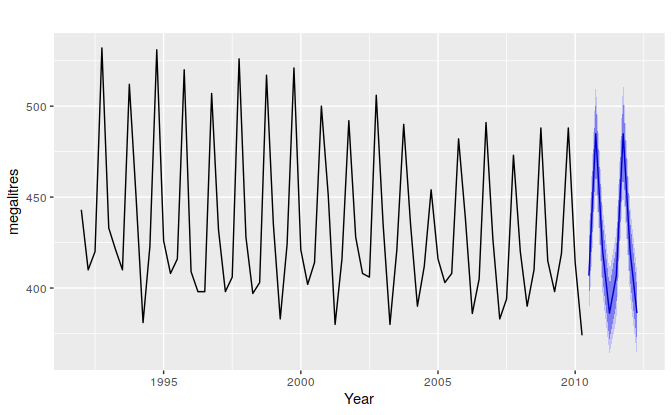
\includegraphics[width=0.7\linewidth]{forecast}
	\caption{Forecast of production of beer in Australia}
	\label{fig:forecast}
\end{figure}
Dark blue lines show the mean forecast \\
Light blue band shows the confidence interval

\end{frame}

\begin{frame}{Three Types of Forecasting Models}
Task: Forecast Electricity Demand at Time T

\begin{enumerate}
	\item Explanatory model \\$E_T = f(Temperature_T, GDP_T, Population_T, Day_T, Month_T, Hour_T)$
	\item Timeseries model \\ $E_T = f(E_{T-1}, E_{T-2}, \cdots)$
	\item Mixed model \\ $E_T = f(E_{T-1}, E_{T-2},Temperature_T, GDP_T, Population_T, \cdots )$
\end{enumerate}
\end{frame}

\begin{frame}{The Importance of Domain Knowledge in Forecasting}
\begin{figure}
	\centering
	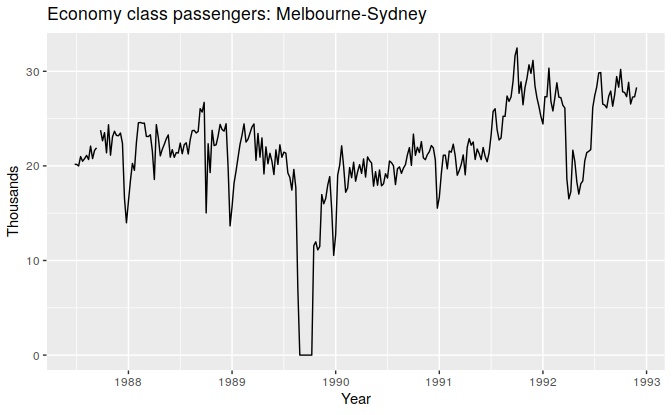
\includegraphics[width=0.4\linewidth]{domain}
	\caption{Weekly economy passenger load on Ansett Airlines.}
	\vspace{-15pt}
	\label{fig:forecast}
\end{figure}
\begin{itemize}
	\item There was a period in 1989 when no passengers were carried
	\item There was a period of reduced load in 1992. This was due to a trial in which some economy class seats were replaced by business class seats.
	\item A large increase in passenger load occurred in the second half of 1991.
	\item There are some large dips in load around the start of each year. These are due to holiday effects.
\end{itemize}

\end{frame}

\begin{frame}{Time Series Patterns}
\begin{figure}
	\centering
	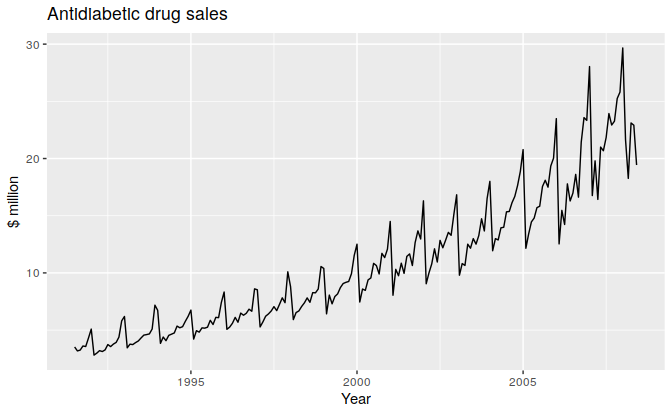
\includegraphics[width=0.6\linewidth]{properties}

	\vspace{-15pt}
	\label{fig:forecast}
\end{figure}

\begin{itemize}
	\item \textbf{Trend}: Long term increase or decrease. 
	\item \textbf{Season}: Time series is affected by seasonal factors such as the time of the year or the day of the week
	\item \textbf{Cyclic}: A cycle occurs when the data exhibit rises and falls that are not of a fixed frequency.
\end{itemize}

\end{frame}

\begin{frame}{Seasonal v/s Cyclic}
\begin{figure}
	\centering
	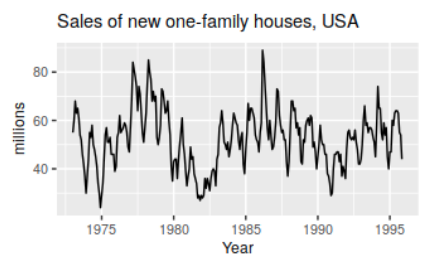
\includegraphics[width=0.6\linewidth]{cyclic-seasonal}
	
	\vspace{-15pt}
	\label{fig:forecast}
\end{figure}

\begin{itemize}
	\item Seasonality: within every year, there is pattern of sales
	\item Cyclic: Every 6 years or so, there is a similar pattern
\end{itemize}
\end{frame}

\begin{frame}{No Pattern in Timeseries}
\begin{figure}
	\centering
	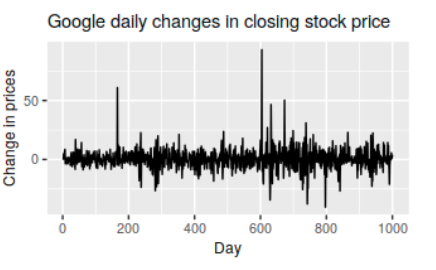
\includegraphics[width=0.6\linewidth]{no-pattern}
	
	\vspace{-15pt}
	\label{fig:forecast}
\end{figure}

\begin{itemize}
	\item Trend: None exists
	\item Seasonality: None exists
	\item Cyclic: None exists
\end{itemize}
Thus, very difficult to forecast
\end{frame}

\begin{frame}{Simple Forecasting Methods}
\begin{itemize}
	\item Average method: $\hat{y}_{T+h}|y_{1:T} = \frac{\sum_{t =1}^{T}y_t}{T}$
	\item Naive method: $\hat{y}_{T+h}|y_{1:T} = y_T$
	\item Seasonal naive method: 
	\begin{itemize}
		\item Same as naive method, but, incorporates seasonal information, e.g. Forecast is the same as the value in the same month last year.
		\item $\hat{y}_{T+h}|{y_{1:T}} = y_{T+h-m(k+1)}$
		where $m$ is the seasonal period and $k$ is is the integer part of $\frac{(h-1)}{m}$ 
		\item Let us assume we are forecasting monthly and we want to forecast for Mar 2020 (month=3) and current time is Jan 2020 (month=1). Thus, $h=2$. Let us assume yearly seasonality, i.e. $m=12$. Thus, prediction for Mar 2020 is value at (Jan+2 months) - $12\times {2-1}\%{12} = $Mar 2020 - 12 Months = Mar 2019
	\end{itemize} 
	
\end{itemize}


\end{frame}

\begin{frame}{Simple Forecasting Methods}
\begin{figure}
	\centering
	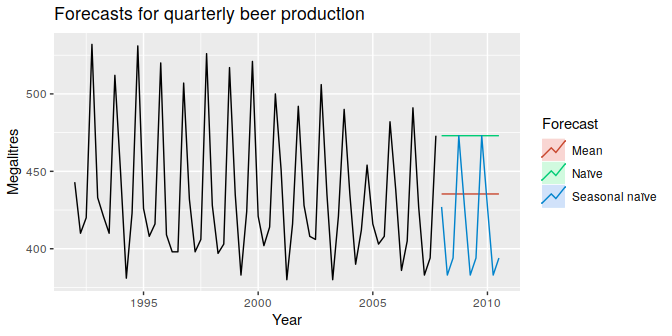
\includegraphics[width=0.9\linewidth]{forecast-naive}
	
	\vspace{-15pt}
	\label{fig:forecast}
\end{figure}

Learning: Simple solutions often work well, especially if you know about the domain.
\end{frame}

\begin{frame}{Evaluating Forecast Accuracy}
\begin{figure}
	\centering
	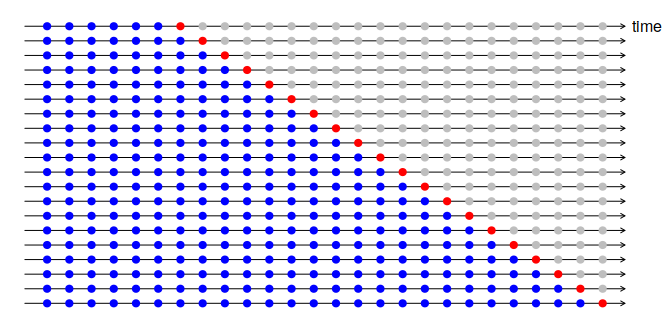
\includegraphics[width=1\linewidth]{timseries-cv1}
	\caption{Timeseries cross-validation for $1$ timestep ahead prediction}
	\vspace{-15pt}
	\label{fig:timeseries-cv}
\end{figure}
Question: How do you nested CV? \\
Answer: Similarly divide the train into train and validation preserving the notion of timeseries.
\end{frame}

\begin{frame}{Evaluating Forecast Accuracy}
\begin{figure}
	\centering
	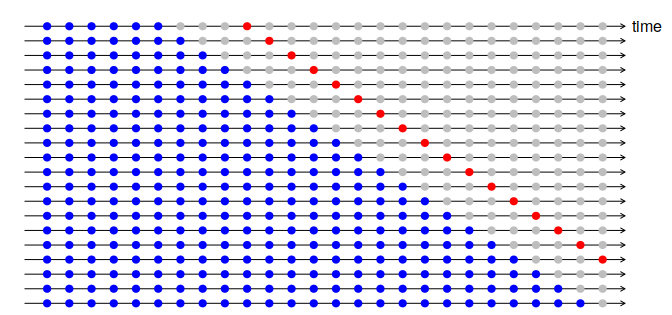
\includegraphics[width=1\linewidth]{timseries-cv2}
	\caption{Timeseries cross-validation for $k=4$ timestep ahead prediction}
	\vspace{-15pt}
	\label{fig:timeseries-cv}
\end{figure}

\end{frame}

\begin{frame}{Stationarity}
\begin{itemize}
	\item A stationary time series is one whose properties do not depend on the time at which the series is observed
	\item Time series with trends, or with seasonality, are not stationary 
	\item White noise series is stationary — it does not matter when you observe it, it should look much the same at any point in time.
\end{itemize}
\end{frame}


\begin{frame}{Stationarity: Which of these are stationary?}
\begin{figure}
	\centering
	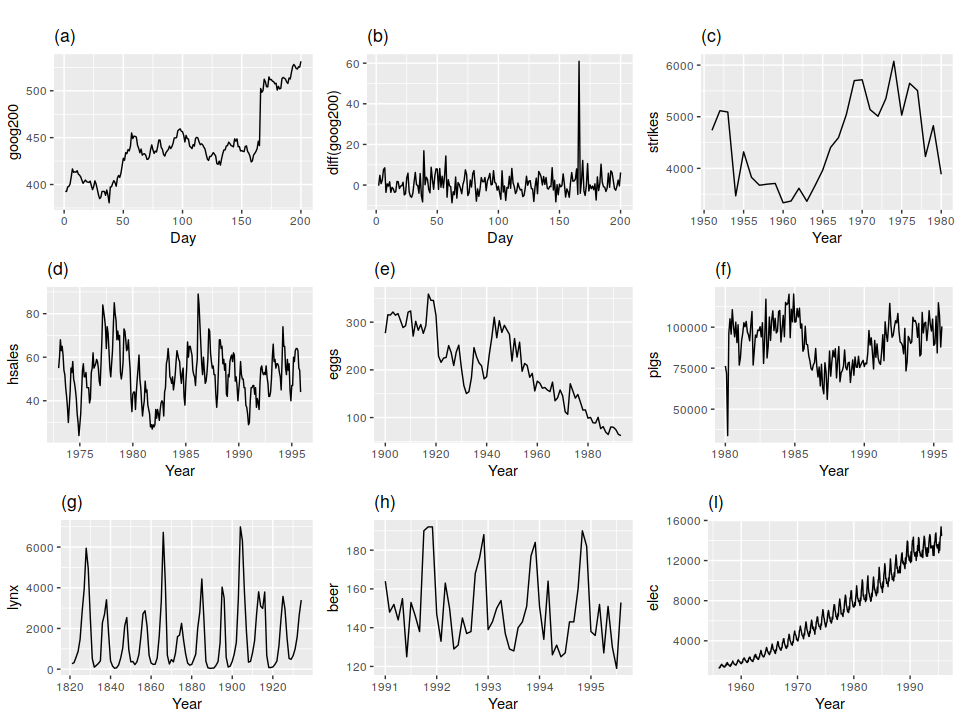
\includegraphics[width=0.6\linewidth]{stationary}
	\vspace{-15pt}
	\label{fig:timeseries-cv}
\end{figure}
\begin{itemize}
	\item Series with trends: a, c, e, f, i
	\item Series with seasonality: d, h, i
	\item Stationary: b and g (cycles are aperiodic)
\end{itemize}
\end{frame}

\begin{frame}{Differencing}
\begin{figure}
	\centering
	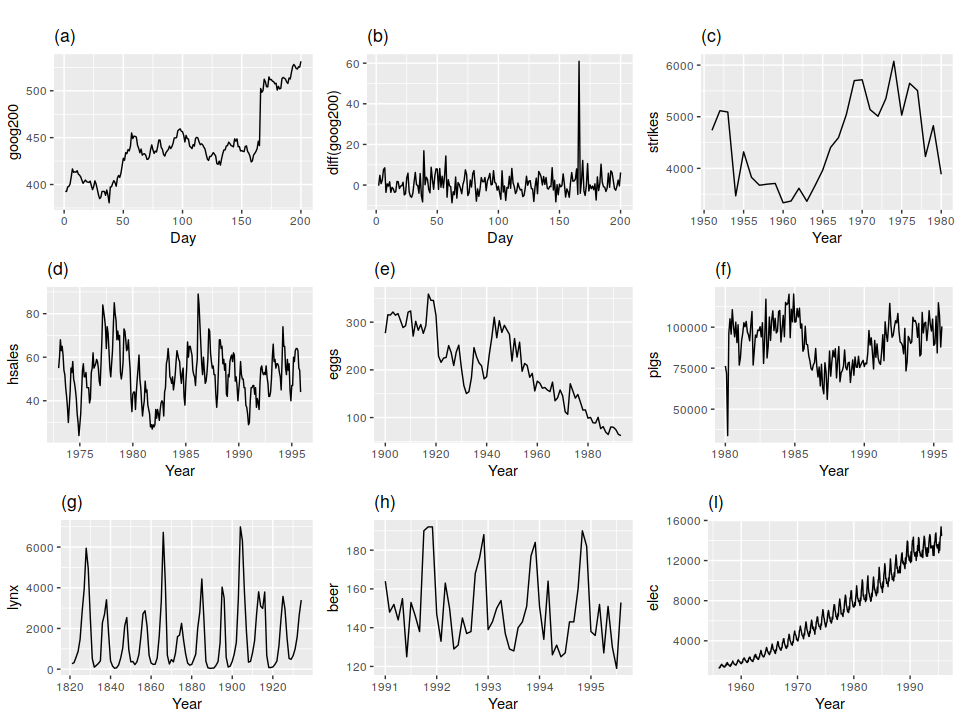
\includegraphics[width=0.6\linewidth]{stationary}
	\vspace{-15pt}
	\label{fig:timeseries-cv}
\end{figure}
What is the relation between a and b? \\
b is the first order time difference of a! \\
b is stationary, while a is not!
\end{frame}

\begin{frame}{Differencing}
\begin{figure}
	\centering
	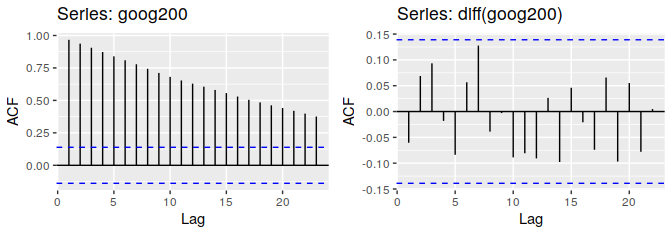
\includegraphics[width=0.9\linewidth]{acfstationary}
	\vspace{-15pt}
	\label{fig:timeseries-cv}
\end{figure}
For (a) the ACF is significant \\
For (b), the ACF declines rapidly
\end{frame}

\begin{frame}{Autoregression}
$y_{t} = c + \phi_{1}y_{t-1} + \phi_{2}y_{t-2} + \dots + \phi_{p}y_{t-p} + \varepsilon_{t},$where $\varepsilon_{t}$ 

is white noise.
\end{frame}

\end{document}